% ---------------------------------------------------------------- 4 method
\section{Proposed DN-SC Framework}
\label{sec:method}

This section develops the DN-SC transceiver. It first describes the rate-nested codebook and its power control, then the Bayesian receiver with its language prior, the time-nested memories and their synchronization, and the token-level refinement protocol. It closes with the cost model and the analytical properties on which the evaluation relies. Figure~\ref{fig:architecture} shows the architecture of the transceiver.

\begin{figure}[!tbp]
\centering
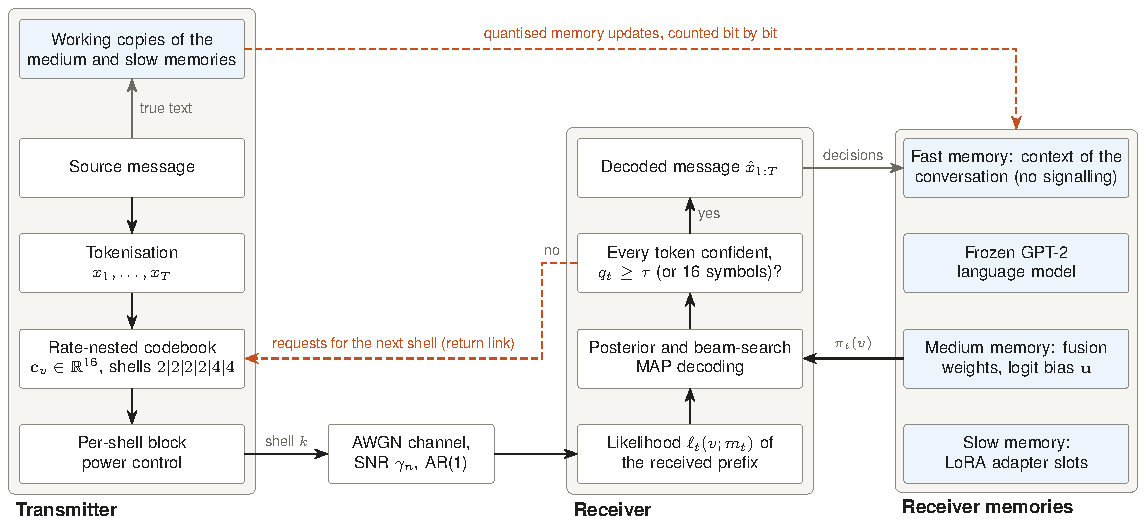
\includegraphics[width=\linewidth]{diagrams/fig_architecture.pdf}
\caption{Architecture of DN-SC. Solid arrows denote the forward data path; dashed arrows denote the return-link requests for further shells and the shipments that synchronize the medium and slow memories of the receiver, both of which are charged in channel symbols. The fast memory (context) is built by the receiver from its own decisions and requires no signaling.}
\label{fig:architecture}
\end{figure}

\subsection{Rate-Nested Codebook and Block Power Control}
\label{sec:method-codebook}

Let $\vect{e}_v\in\R^{D}$ denote the input embedding of token $v$ in the frozen language model and $s_e$ the standard deviation of all entries of the embedding table. A small network maps the scaled embedding $\bar{\vect{e}}_v = \vect{e}_v/s_e$ to a raw codeword,
\begin{equation}
\tilde{\vect{c}}_v = \vect{W}_1\bar{\vect{e}}_v + \vect{W}_3\,\GELU\!\left(\vect{W}_2\bar{\vect{e}}_v + \vect{b}_2\right),
\label{eq:codeword}
\end{equation}
with $\vect{W}_1\in\R^{M\times D}$, $\vect{W}_2\in\R^{H\times D}$, $\vect{b}_2\in\R^{H}$ and $\vect{W}_3\in\R^{M\times H}$. Since $\vect{W}_3$ is initialized at zero, training starts from a linear projection of the embeddings, and no language model has to run at the transmitter to encode. The $M$ coordinates are partitioned into $K$ shells at the prefix lengths $m_1<m_2<\dots<m_K = M$; shell $k$ holds the coordinates $\mathcal{S}_k = \{m_{k-1}+1,\dots,m_k\}$, with $m_0 = 0$, and has width $d_k = m_k-m_{k-1}$. Each shell is centered and scaled under the unigram distribution $q$ of the base corpus,
\begin{equation}
\hat{\vect{c}}_{v,k} = \frac{\tilde{\vect{c}}_{v,\mathcal{S}_k}-\vect{\mu}_k}{\sqrt{P_k}},\qquad
\vect{\mu}_k = \sum_{v\in\mathcal{V}} q(v)\,\tilde{\vect{c}}_{v,\mathcal{S}_k},\qquad
P_k = \frac{1}{d_k}\sum_{v\in\mathcal{V}} q(v)\,\bigl\lVert\tilde{\vect{c}}_{v,\mathcal{S}_k}-\vect{\mu}_k\bigr\rVert^2,
\label{eq:shell}
\end{equation}
and the energy of every codeword in the shell is limited to $\eta$ times the shell average,
\begin{equation}
\vect{c}_{v,\mathcal{S}_k} = \min\!\left\{1,\frac{\sqrt{\eta\,d_k}}{\lVert\hat{\vect{c}}_{v,k}\rVert}\right\}\hat{\vect{c}}_{v,k}.
\label{eq:peak}
\end{equation}
Every shell therefore has zero mean before the peak limit and an average power of at most one per symbol under $q$.

This constraint holds on average over the base corpus, not for a particular message. Before transmission, shell $k$ of the set $\mathcal{T}$ of tokens of a message that a round carries, namely all $T$ tokens in the first round and the requested tokens in a refinement round, is therefore multiplied by
\begin{equation}
g_k(\mathcal{T}) = \left(\frac{|\mathcal{T}|\,d_k}{\sum_{t\in\mathcal{T}}\lVert\vect{c}_{x_t,\mathcal{S}_k}\rVert^2}\right)^{1/2},
\label{eq:gain}
\end{equation}
so that every transmitted block has an average power of exactly one per symbol. The gain is applied to the whole block, pilots included, and is absorbed into the channel estimate; the receiver observes it only through the precision $\lambda_{t,j}$ in~(\ref{eq:channel}). Consequently, no receiver can gain power from content whose codewords happen to be large.

\emph{Property 1 (exact incremental refinement).} Every transmitted block satisfies the power constraint with equality, and hence so does every prefix. Receiving shells $1,\dots,k$ of all tokens in $k$ separate rounds yields observations with the same distribution as receiving the prefix of length $m_k$ at once, and a refinement round extends the prefix of each requested token by one shell, received with the precision determined by the gain of the requested set.

\emph{Proof.} By~(\ref{eq:gain}), the gain of a block depends only on the coordinates of its own shell and on the tokens it carries, and by~(\ref{eq:channel}) the noise is independent across symbols. Neither a block nor its noise therefore depends on when, or whether, other shells are transmitted. Since each block has unit average power per symbol, the average over the blocks of any prefix is also one. $\square$

The codebook is trained once, before deployment and without the language model, by maximizing the channel-only posterior of the transmitted token at randomly drawn prefix lengths and SNRs,
\begin{equation}
\mathcal{L}_\mathrm{cb}(\vect{W}) = \E_{v\sim\bar{q},\;\gamma\sim\mathcal{U}[\gamma_\mathrm{lo},\gamma_\mathrm{hi}],\;\vect{w}}\left[\frac{1}{|\mathcal{M}_b|}\sum_{m\in\mathcal{M}_b}-\log\frac{\exp\ell(v;m)}{\sum_{v'\in\mathcal{V}}\exp\ell(v';m)}\right],
\label{eq:codebook-loss}
\end{equation}
where $\ell$ is the log-likelihood~(\ref{eq:likelihood}) below with $\lambda_{t,j} = 10^{\gamma/10}$, $\mathcal{M}_b$ is a set of prefix lengths drawn afresh for every batch, and $\bar{q}$ mixes the unigram distribution of the base corpus with the uniform distribution over $\mathcal{V}$, so that tokens absent from the base corpus, which form the vocabulary of later domains, are also separated. Because all prefixes are trained jointly, each prefix constitutes a usable code.

\subsection{Bayesian Receiver With a Language Prior}
\label{sec:method-receiver}

When the first $m$ symbols of token $t$ have been received, the Gaussian log-likelihood of every vocabulary entry follows from~(\ref{eq:channel}), up to a term that does not depend on $v$, as
\begin{equation}
\ell_t(v;m) = \sum_{j=1}^{m}\lambda_{t,j}\left(y_{t,j}\,c_{v,j}-\tfrac{1}{2}\,c_{v,j}^2\right),
\label{eq:likelihood}
\end{equation}
which is evaluated for all $V$ entries by one matrix product of the received symbols with the codebook. The prior is the frozen language model, modified by the memories of the receiver. The slow memory consists of $K_\mathrm{s}$ LoRA adapters; adapter $s$ replaces each adapted weight matrix $\vect{W}^{(i)}$ of the language model by
\begin{equation}
\vect{W}^{(i)}_s = \vect{W}^{(i)} + \frac{\alpha}{r}\,\vect{B}^{(i)}_s\vect{A}^{(i)}_s,\qquad \vect{A}^{(i)}_s\in\R^{r\times D_\mathrm{in}},\quad \vect{B}^{(i)}_s\in\R^{D_\mathrm{out}\times r},
\label{eq:lora}
\end{equation}
with rank $r$ and scaling $\alpha$ \cite{hu2022lora}, and $\phi_s = \{\vect{A}^{(i)}_s,\vect{B}^{(i)}_s\}_i$ denotes the parameters of slot $s$ ($\phi_\varnothing$: no adapter). With $\hat{\vect{x}}_{<t}$ the tokens already decided in the message and $\vect{h}$ the context, the prior of the receiver is
\begin{equation}
\log\pi_t(v) = \log\softmax_v\!\left[\,w_\mathrm{p}\log p_{\theta}\!\left(v\mid\vect{h},\hat{\vect{x}}_{<t};\phi_s\right) + \frac{1}{s_e}\,\vect{e}_v^{\top}\vect{u}\,\right],
\label{eq:prior}
\end{equation}
where the weight $w_\mathrm{p}$ sharpens or flattens the language model and $\vect{u}\in\R^{D}$ defines a logit bias in embedding space, which shifts the probability of all tokens that are close in meaning by means of a single vector. The posterior of token $t$ after $m_t$ symbols, the decision and the receiver's confidence in it are
\begin{equation}
p_t(v) = \frac{\pi_t(v)\,e^{w_\mathrm{l}\ell_t(v;m_t)}}{Z_t},\qquad
Z_t = \sum_{v'\in\mathcal{V}}\pi_t(v')\,e^{w_\mathrm{l}\ell_t(v';m_t)},\qquad
\hat{x}_t = \argmax_{v}\,p_t(v),\qquad q_t = \max_{v}\,p_t(v),
\label{eq:posterior}
\end{equation}
with a likelihood weight $w_\mathrm{l}$; before any adaptation, $w_\mathrm{p} = w_\mathrm{l} = 1$ and $\vect{u} = \vect{0}$.

Decoding is free-running, that is, the language model is conditioned on the receiver's own earlier decisions, so that an early error misleads the prior for the remainder of the sentence. The receiver therefore approximates the sequence maximum a posteriori (MAP) decision
\begin{equation}
\hat{\vect{x}} = \argmax_{\vect{x}\in\mathcal{V}^T} J(\vect{x}),\qquad
J(x_{1:t}) = \sum_{i=1}^{t}\Bigl[\log\pi_i(x_i\mid x_{<i}) + w_\mathrm{l}\,\ell_i(x_i;m_i)\Bigr],
\label{eq:map}
\end{equation}
in which $J$ equals the log-posterior of the partial sentence up to a constant, by a beam search of width $B$ that retains, at every position, the $B$ best extensions of the surviving partial sentences,
\begin{equation}
\mathcal{B}_t = \operatorname*{top-}B_{\,(x_{1:t-1},v)\,:\;x_{1:t-1}\in\mathcal{B}_{t-1},\;v\in\mathcal{V}}\; J(x_{1:t-1},v),\qquad \mathcal{B}_0 = \{\varnothing\}.
\label{eq:beam}
\end{equation}
The ranking must use the joint score $J$. Summing the per-position posteriors of~(\ref{eq:posterior}) instead gives
\begin{equation}
\sum_{i=1}^{t}\log p_i(x_i) = J(x_{1:t}) - \sum_{i=1}^{t}\log Z_i(x_{<i}),
\label{eq:labelbias}
\end{equation}
where $Z_i(x_{<i})$ is proportional to the predictive likelihood of the observation of position $i$ given the prefix. Such a ranking penalizes exactly those prefixes under which the next observation is well explained, which is a form of the label-bias problem \cite{lafferty2001}. The confidence $q_t$ reported for a decision is that of the posterior at position $t$ along the selected path.

\subsection{Time-Nested Memories and Their Synchronization}
\label{sec:method-memories}

The prior~(\ref{eq:prior}) is shaped by three memories that change at three rates (Figure~\ref{fig:protocol}b). The fast memory is the context: a message that continues a document is decoded with the receiver's own reconstruction of the preceding messages of the conversation as $\vect{h}$, up to a fixed number of tokens. This is the native memory of the language model; it changes with every message, requires no gradient and costs nothing on the air, but its errors propagate, since a wrongly decoded message becomes a wrong context.

The medium memory $\phi_\mathrm{med} = (w_\mathrm{p}, w_\mathrm{l}, \vect{u})$ and the slow memory $\phi_\mathrm{slow} = \{\phi_1,\dots,\phi_{K_\mathrm{s}}\}$ can only be learned with the true text. They are therefore learned at the transmitter, which maintains a working copy $\phi^\mathrm{tx}$ of both and, at every adaptation step $n$, evaluates the posterior cross-entropy of the $N_n$ tokens of the step's messages with the true earlier tokens and the true context $\vect{h}^\mathrm{tx}_i$,
\begin{equation}
\mathcal{L}_n(\phi) = \frac{1}{|\mathcal{M}_n|}\sum_{m\in\mathcal{M}_n}\frac{1}{N_n}\sum_{(i,t)}-\log p_{t}^{\phi}\!\left(x_{i,t}\mid \vect{y}_{i,t,1:m},\,\vect{x}_{i,<t},\,\vect{h}_i^\mathrm{tx}\right),
\label{eq:adapt-loss}
\end{equation}
averaged over the operating prefix length and one further prefix length drawn at random ($\mathcal{M}_n$), so that the prior serves every rate. Each level $\ell\in\{\mathrm{med},\mathrm{slow}\}$ takes one optimizer step per adaptation step with its own learning rate $\eta_\ell$,
\begin{equation}
\phi^\mathrm{tx}_{\ell,n} = \phi^\mathrm{tx}_{\ell,n-1} - \eta_\ell\,\mathrm{Adam}\!\left(\nabla_{\phi_\ell}\mathcal{L}_n\right),
\label{eq:adam}
\end{equation}
and within the slow memory only the active slot is updated. The receiver holds its own copy $\phi^\mathrm{rx}_\ell$, which changes only at the period $C_\ell$ of the level. When $n\equiv 0 \pmod{C_\ell}$, the transmitter quantizes the difference $\vect{\Delta} = \phi^\mathrm{tx}_\ell-\phi^\mathrm{rx}_\ell$ of every parameter tensor with $b$ bits per entry, and both ends apply the quantized difference:
\begin{equation}
\mathcal{Q}_b(\vect{\Delta}) = \frac{a}{L}\,\mathrm{round}\!\left(\frac{L\,\vect{\Delta}}{a}\right),\qquad a = \lVert\vect{\Delta}\rVert_\infty,\qquad L = 2^{b-1}-1,\qquad
\phi^\mathrm{rx}_\ell \leftarrow \phi^\mathrm{rx}_\ell + \mathcal{Q}_b(\vect{\Delta}),\qquad \phi^\mathrm{tx}_\ell \leftarrow \phi^\mathrm{rx}_\ell .
\label{eq:sync}
\end{equation}
Between two shipments the receiver decodes with a stale copy,
\begin{equation}
\phi^\mathrm{rx}_\ell(n) = \phi^\mathrm{rx}_\ell\!\left(C_\ell\left\lfloor n/C_\ell\right\rfloor\right),
\label{eq:stale}
\end{equation}
so that the period $C_\ell$ trades staleness against air time; all receivers compared in this article learn in the same way and differ only in when each level reaches the receiver. A shipment of level $\ell$ costs $B_\ell = \sum_{i\in\ell}(32 + b\,n_i)$ bits, where $n_i$ is the number of entries of tensor $i$ and 32 bits carry its scale $a$ (an all-zero difference costs a single flag bit), and the slot choice described below costs $\lceil\log_2(K_\mathrm{s}+1)\rceil$ bits every $C_\mathrm{sel}$ steps. The average synchronization rate is therefore
\begin{equation}
\bar{B}_\mathrm{sync} = \frac{B_\mathrm{med}}{C_\mathrm{med}} + \frac{B_\mathrm{slow}}{C_\mathrm{slow}} + \frac{\lceil\log_2(K_\mathrm{s}+1)\rceil}{C_\mathrm{sel}}\quad\text{bits per adaptation step}.
\label{eq:syncrate}
\end{equation}
The multi-frequency organization follows the nested-learning view \cite{behrouz2025}, and the quantized, bit-counted synchronization follows the practice of communication-efficient learning \cite{alistarh2017,mcmahan2017}.

\emph{Proposition 2 (synchronization).} Immediately after a shipment of level $\ell$, the two copies are bit-identical, and every entry of the applied difference deviates from the unquantized difference by at most $a/(2L)$. If only the active slot of the slow memory changes between two shipments, the average number of synchronized bits per adaptation step equals~(\ref{eq:syncrate}).

\emph{Proof.} Both ends add the same quantized difference to the same copy, and the transmitter then resets its working copy to the result, which proves the first claim. Rounding to the grid $\{ja/L\}$ moves every entry by at most half a grid step, which proves the second. In each period of length $C_\ell$ exactly one shipment of cost $B_\ell$ occurs, because only one tensor set per level has changed, and the slot choice is signaled once every $C_\mathrm{sel}$ steps; averaging over the steps gives~(\ref{eq:syncrate}). $\square$

Adapting a single adapter to one domain can damage the prior for another, so the slow memory keeps one adapter per domain. Every $C_\mathrm{sel}$ steps, the transmitter evaluates, on the messages it is about to send, the prior cross-entropy $H_s$ in bits per token of the receiver's copy with every choice $s\in\{\varnothing,1,\dots,K_\mathrm{s}\}$, and changes the active slot $s_\mathrm{cur}$ only if another choice is better by a margin $\delta$:
\begin{equation}
s^\star = \argmin_{s}\,H_s,\qquad
s_\mathrm{new} = \begin{cases} s^\star, & H_{s^\star} < H_{s_\mathrm{cur}}-\delta,\\ s_\mathrm{cur}, & \text{otherwise}.\end{cases}
\label{eq:slot}
\end{equation}
Whenever $s_\mathrm{new} = \varnothing$ and an untrained slot remains, that slot is started instead. A domain that returns therefore finds its adapter intact, recalling it costs two bits rather than a new synchronization, and the receiver keeps an adapter that is worse than none by more than $\delta$ for at most $C_\mathrm{sel}$ steps. Algorithm~\ref{alg:step} states one adaptation step, and Figure~\ref{fig:flowstep} depicts it as a flowchart.

\begin{algorithm}[!tbp]
\caption{One adaptation step $n$ of DN-SC}
\label{alg:step}
\small
\begin{algorithmic}[1]
\Require messages $\vect{x}_1,\dots,\vect{x}_{N_\mathrm{c}}$ of the step; SNR $\gamma_n$; receiver copies $\phi^\mathrm{rx}$ and contexts $\vect{h}^\mathrm{rx}_i$; transmitter copies $\phi^\mathrm{tx}$ and contexts $\vect{h}^\mathrm{tx}_i$
\Ensure decoded messages $\hat{\vect{x}}_i$; updated memories; bit ledger
\If{$(n-1)\bmod C_\mathrm{sel} = 0$} \Comment{slot choice, Eq.~(\ref{eq:slot})}
  \State evaluate $H_s$ under $\phi^\mathrm{rx}$, choose $s_\mathrm{new}$ and signal it; ledger $\mathrel{+}= \lceil\log_2(K_\mathrm{s}+1)\rceil$
\EndIf
\For{each message $i$} \Comment{transmission and decoding}
  \State encode $\vect{x}_i$ by Eqs.~(\ref{eq:codeword})--(\ref{eq:gain}) and send round 1, $m_{k_0}$ symbols per token
  \Repeat
    \State decode by beam search, Eqs.~(\ref{eq:likelihood})--(\ref{eq:beam}), with prior $\phi^\mathrm{rx}$ and context $\vect{h}^\mathrm{rx}_i$
    \State close every open token with $q_t\ge\tau$; request the next shell for the others \Comment{Eqs.~(\ref{eq:stop}), (\ref{eq:feedback})}
    \State send the next shell of the requested tokens at unit power, Eq.~(\ref{eq:gain})
  \Until{no token is open}
  \State $\vect{h}^\mathrm{rx}_i \leftarrow \vect{h}^\mathrm{rx}_i\Vert\hat{\vect{x}}_i$; \quad $\vect{h}^\mathrm{tx}_i \leftarrow \vect{h}^\mathrm{tx}_i\Vert\vect{x}_i$ \Comment{fast memory}
\EndFor
\State update $\phi^\mathrm{tx}_\mathrm{med}$ and the active slot of $\phi^\mathrm{tx}_\mathrm{slow}$ by Eqs.~(\ref{eq:adapt-loss}) and (\ref{eq:adam})
\For{$\ell\in\{\mathrm{med},\mathrm{slow}\}$ with $n\equiv 0\pmod{C_\ell}$}
  \State ship $\mathcal{Q}_b(\phi^\mathrm{tx}_\ell-\phi^\mathrm{rx}_\ell)$ and set both copies equal; ledger $\mathrel{+}= B_\ell$ \Comment{Eq.~(\ref{eq:sync})}
\EndFor
\end{algorithmic}
\end{algorithm}

\begin{figure}[!tbp]
\centering
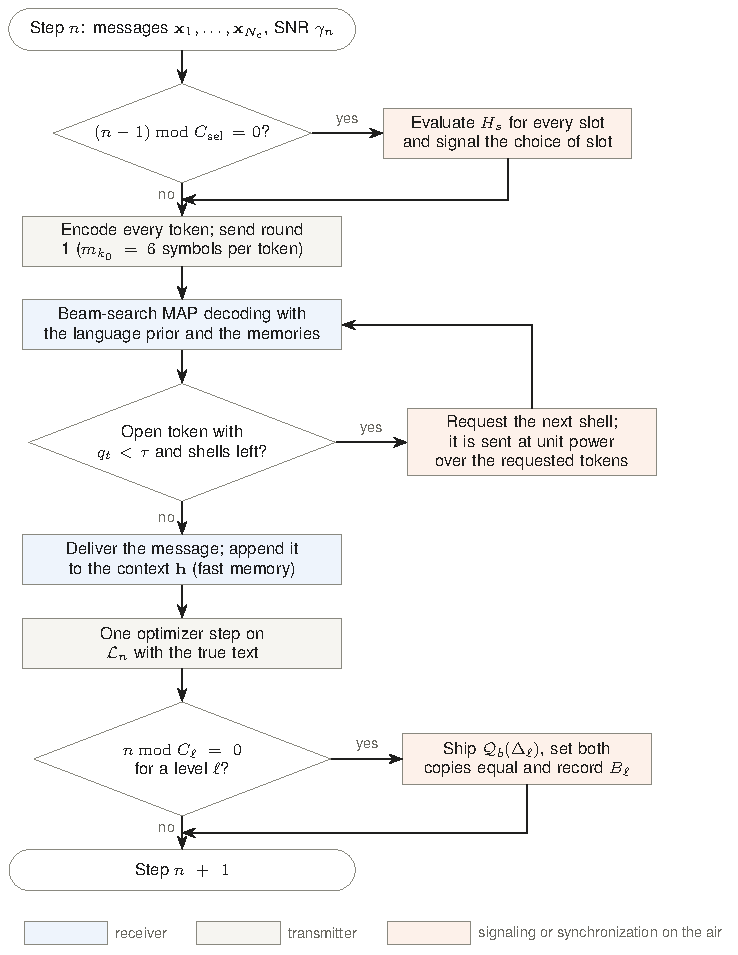
\includegraphics[width=0.7\linewidth]{diagrams/fig_flow_step.pdf}
\caption{Flowchart of one adaptation step of DN-SC (Algorithm~\ref{alg:step}). Tx and Rx indicate the end at which an operation is performed; parallelograms denote transmissions of signaling or synchronization data.}
\label{fig:flowstep}
\end{figure}

\subsection{Token-Level Selective Refinement}
\label{sec:method-refinement}

Round 1 delivers the first $m_{k_0}$ symbols of every token. After each round, the receiver decodes the whole message again with the symbols received so far and decides, for every token that is still open, whether to request its next shell. A token that is not continued is closed permanently, and no decision is required after the last shell (Figure~\ref{fig:protocol}a). Under this rule, token $t$ stops at the shell
\begin{equation}
k_t(\tau) = \min\left\{k\in\{k_0,\dots,K\}: q_t^{(k)}\ge\tau\right\}\quad(\text{or } K \text{ if no such } k\text{ exists}),\qquad
S_\mathrm{fwd}(\tau) = \frac{1}{N_\mathrm{tok}}\sum_{t} m_{k_t(\tau)},
\label{eq:stop}
\end{equation}
where $q_t^{(k)}$ is the confidence of token $t$ when the message is decoded with $m_k$ symbols for that token, and $S_\mathrm{fwd}$ is the mean number of forward symbols per token over the $N_\mathrm{tok}$ tokens of an adaptation step; operating curves average these step means over the steps. By Property 1, the additional symbols extend what has already been received, which constitutes incremental redundancy at the level of individual tokens, spent where the language model cannot fill the gap.

\begin{figure}[!tbp]
\centering
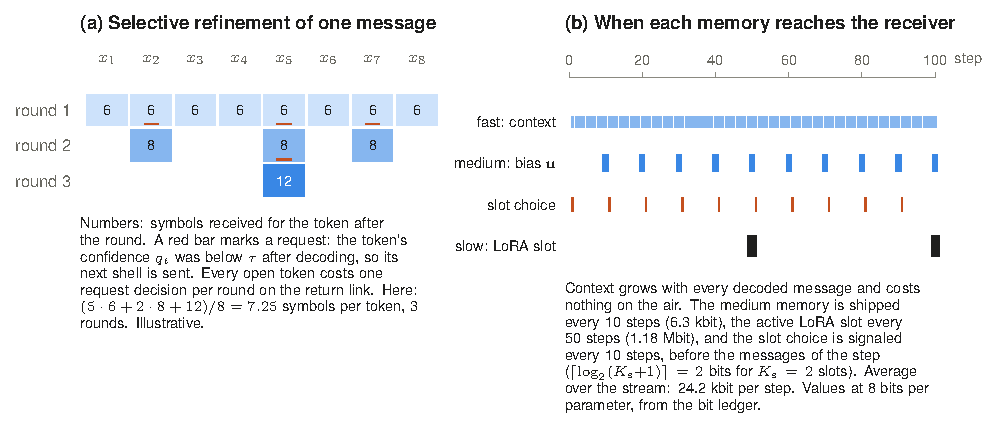
\includegraphics[width=\linewidth]{diagrams/fig_protocol.pdf}
\caption{(a) Selective refinement of one message of eight tokens with a first round of 6 symbols per token (illustrative). Each cell gives the number of symbols received for the token after the round, and each arrow a request for the next shell on the return link; the mean cost is $(5\cdot 6+2\cdot 8+12)/8 = 7.25$ symbols per token in three rounds. (b) Instants at which each memory reaches the receiver during the first 100 adaptation steps, with the cost of one shipment at $b = 8$ bits per parameter; averaged over the stream, the synchronization amounts to 24.2\,kbit per adaptation step (bit ledger of the experiments).}
\label{fig:protocol}
\end{figure}

Let $n_r$ denote the number of tokens that are open after round $r$ and must be decided upon, and $c_r\le n_r$ the number of them that are continued. Two costs of the requests are derived from the decisions actually taken, in bits per token, namely an explicit bitmap and the empirical entropy of the decisions of each round, which an ideal entropy coder of the bitmap would approach:
\begin{equation}
B_\mathrm{bm} = \frac{1}{N_\mathrm{tok}}\sum_{r} n_r,\qquad
B_\mathrm{H} = \frac{1}{N_\mathrm{tok}}\sum_{r} n_r\,h_2\!\left(\frac{c_r}{n_r}\right),\qquad
h_2(p) = -p\log_2 p-(1-p)\log_2(1-p).
\label{eq:feedback}
\end{equation}
Both are converted into real channel symbols at $C(\bar{\gamma})$ and added to the forward symbols. The entropy $B_\mathrm{H}$ is a lower reference rather than an implemented code, whereas the bitmap is directly implementable; a fixed-prefix receiver requires no signaling at all.

\emph{Proposition 3 (signaling bounds).} For every threshold $\tau$, $0\le B_\mathrm{H}\le B_\mathrm{bm}\le K-k_0$ bits per token.

\emph{Proof.} Since $0\le h_2(p)\le 1$, $B_\mathrm{H}\le B_\mathrm{bm}$. A token takes part in one decision after each round in which it is open and has a shell left, which happens at most $K-k_0$ times; summing over tokens gives $\sum_r n_r\le (K-k_0)N_\mathrm{tok}$. $\square$

\subsection{Cost Model and Analytical Properties}
\label{sec:method-cost}

Each receiver is characterized by its measured operating curve $\{(S_i,A_i)\}$, the cost against the accuracy over the thresholds $\tau$ or the prefix lengths, sorted by cost. The cost at the target accuracy is read by linear interpolation,
\begin{equation}
S(\alpha^\star) = S_i + \frac{\alpha^\star - A_i}{A_{i+1}-A_i}\,\bigl(S_{i+1}-S_i\bigr)\quad\text{for } A_i < \alpha^\star \le A_{i+1},
\label{eq:readoff}
\end{equation}
and, when even the cheapest point of a curve exceeds the target ($A_1\ge\alpha^\star$), at that point, $S(\alpha^\star) = S_1$, which is then an upper bound of the cost at the target. Let $R = \bar{T}\,[S_\mathrm{fwd}+B_\mathrm{fb}/C(\bar{\gamma})]$ be the resulting payload of a receiver per message. If one adaptation step, with $\bar{B}_\mathrm{sync}$ synchronized bits, serves $N$ messages, the net semantic rate and the traffic above which the receiver is cheaper than a reference receiver with payload $R^\mathrm{ref}>R$ and no synchronization are
\begin{equation}
R_\mathrm{net}(N) = R + \frac{\bar{B}_\mathrm{sync}}{C(\bar{\gamma})\,N}\quad\text{real symbols per message},
\label{eq:netrate}
\end{equation}
\begin{equation}
N^\star = \frac{\bar{B}_\mathrm{sync}}{C(\bar{\gamma})\left(R^\mathrm{ref}-R\right)} .
\label{eq:crossover}
\end{equation}
Equation~(\ref{eq:netrate}) is~(\ref{eq:cost}) multiplied by $\bar{T}$.

\emph{Proposition 4 (crossover).} $R_\mathrm{net}(N)$ decreases strictly in $N$, $R_\mathrm{net}(N) < R^\mathrm{ref}$ if and only if $N > N^\star$, and the relative change $R_\mathrm{net}(N)/R^\mathrm{ref} - 1$ tends to $R/R^\mathrm{ref}-1$ as $N\to\infty$.

\emph{Proof.} The second term of~(\ref{eq:netrate}) is positive and inversely proportional to $N$. The inequality $R + \bar{B}_\mathrm{sync}/(C N) < R^\mathrm{ref}$ rearranges to $N > N^\star$, and the limit follows because the second term vanishes. $\square$

The prior cross-entropy~(\ref{eq:metrics}) also determines the cost of an idealized separate design that compresses each token with an arithmetic code matched to the receiver's prior and transmits the compressed bits with a capacity-achieving channel code. Such a design requires on average
\begin{equation}
S_\mathrm{sep} = \frac{\bar{H}}{C(\bar{\gamma})}\quad\text{real symbols per token}
\label{eq:separation}
\end{equation}
for lossless delivery in the limit of long blocks \cite{shannon1948}, so that a reduction $\Delta\bar{H}$ of the prior cross-entropy lowers this benchmark by $\Delta\bar{H}/C(\bar{\gamma})$. The benchmark ignores the penalty of finite block lengths \cite{polyanskiy2010} and the cliff effect at an unknown SNR, and it is used here to relate the knowledge of the receiver to its cost in channel symbols.

The receiver evaluates~(\ref{eq:likelihood}) for all $V$ entries at a cost of $O(Vm)$ operations per token and runs the language model once per token and beam in every decoding pass; selective refinement repeats the pass for the messages that still contain open tokens, so that the number of passes per message equals the number of rounds. The transmitter performs one forward and one backward pass of the language model per adaptation step, the backward pass only through the adapted layers, and one forward pass per candidate slot every $C_\mathrm{sel}$ steps. The codebook is trained once and never shipped. Section~\ref{sec:results-cost} reports the measured parameter counts, latencies and run times.
